\chapteropen{Chapter 13: Equivalence classes and boundary values}{chapter-13}
\markboth{Ch. 13 | EC and BV}{}


\begin{studycolumns}
\vspace{0pt}
\begin{eli5box}
Instead of trying every possible age, sort inputs into buckets that should behave alike. Then test the fence edges: just below, exactly on and just above. If you test two broken fields together, the first error may hide the second, so defensive tests usually break one parameter at a time.
\end{eli5box}
\textbf{Answer check:} State units, representation and inclusive endpoints; partition valid/invalid behaviour, then select full boundary triplets. Combine valid inputs and isolate one invalid parameter per defensive row. Give an oracle. String length, syntax, registration and dependency failures are separate checks.
\end{studycolumns}

\subsection*{Visual: build tests in the right order}
\sectionlabel{h-visual-build-tests-in-the-right-order}


\par\smallskip\noindent\begin{minipage}{\linewidth}\centering
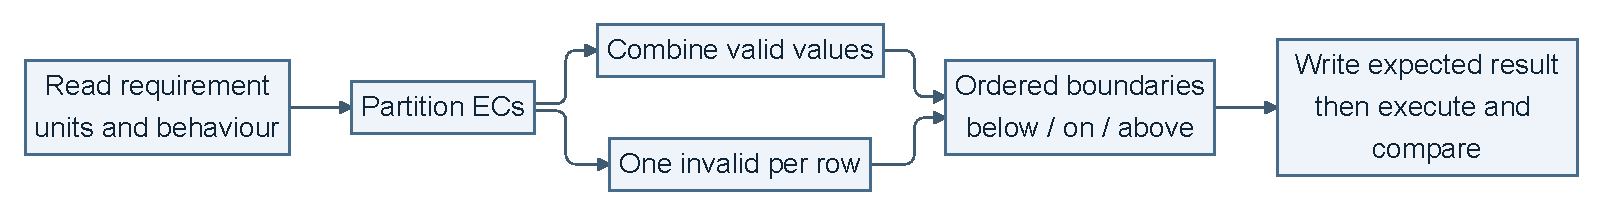
\includegraphics[width=471.96pt]{images/fig-036.pdf}
\captionof{figure}{build tests in the right order}\end{minipage}\par\smallskip

\begin{studycolumns}
\vspace{0pt}



\needspace{4\baselineskip}
\subsection*{13.1 Two assumptions behind black-box testing}
\sectionlabel{h-131-two-assumptions-behind-black-box-testing}
\begin{enumerate}
\item \textbf{A verifiable requirement /\allowbreak{} API specification exists} --- make software testable from inception. \emph{Not verifiable:} "The company must not hire too-young or too-old people." \emph{Verifiable:} "0--15 and 55--99: do not hire; 16--17: part-time; 18--54: full-time."
\item \textbf{The code must be testable} --- a 100-branch \code{if (age=\allowbreak{}=\allowbreak{}0) \ldots{} if (age=\allowbreak{}=\allowbreak{}99)} chain makes black-box testing ineffective compared with range conditions.
\end{enumerate}
\needspace{4\baselineskip}
\subsection*{13.2 Equivalence classes}
\sectionlabel{h-132-equivalence-classes}

\begin{quote}\small\color{navy}
A set of input values forms an \textbf{equivalence class (EC)} if:

\begin{itemize}
\item they are all \textbf{supposed to produce the same output};
\item if one value catches a bug, the others \textbf{probably will too};
\item if one value does not catch a bug, the others \textbf{probably will not either}.
\end{itemize}
\end{quote}
\end{studycolumns}

\Needspace{4\baselineskip}
\subsection*{13.3 Partition rules}
\sectionlabel{h-133-partition-rules}


{\fontsize{9}{11}\selectfont
\begin{longtable}{L{\dimexpr 0.34307\linewidth-8.23pt\relax}L{\dimexpr 0.36021\linewidth-8.64pt\relax}L{\dimexpr 0.29672\linewidth-7.12pt\relax}}
\toprule
\rowcolor{ice}\textbf{Input type} & \textbf{Valid ECs} & \textbf{Invalid ECs} \\
\midrule\endfirsthead
\toprule\rowcolor{ice}\textbf{Input type} & \textbf{Valid ECs} & \textbf{Invalid ECs} \\
\midrule\endhead
\multicolumn{3}{r}{\scriptsize Continued on next page}\\\endfoot
\bottomrule\endlastfoot
\textbf{Range of values} (\code{1500 \ensuremath{\leq} x \ensuremath{\leq} 80000}) & \textbf{ONE} valid EC (or more, if the requirement has several valid ranges --- e.g. hiring rules have 4) & \textbf{TWO} invalid ECs (\code{x \ensuremath{\leq} 1499} and \code{x \ensuremath{\geq} 80001}) \\
\textbf{Discrete values} (applicant type \ensuremath{\in} \{Person\}, property type \ensuremath{\in} \{HDB, Condo\}) & \textbf{ONE} valid EC (the listed set) & \textbf{ONE} invalid EC (everything else) \\
\end{longtable}
}

Worked partitions:




{\fontsize{9}{11}\selectfont
\begin{longtable}{L{\dimexpr 0.34550\linewidth-8.29pt\relax}L{\dimexpr 0.31302\linewidth-7.51pt\relax}L{\dimexpr 0.34148\linewidth-8.20pt\relax}}
\toprule
\rowcolor{ice}\textbf{Parameter} & \textbf{Valid EC(s)} & \textbf{Invalid EC(s)} \\
\midrule\endfirsthead
\toprule\rowcolor{ice}\textbf{Parameter} & \textbf{Valid EC(s)} & \textbf{Invalid EC(s)} \\
\midrule\endhead
\multicolumn{3}{r}{\scriptsize Continued on next page}\\\endfoot
\bottomrule\endlastfoot
Mortgage income (1500--80000) & 1500 \ensuremath{\leq} x \ensuremath{\leq} 80000 & x \ensuremath{\leq} 1499 ; x \ensuremath{\geq} 80001 \\
\#mortgages (0--5) & 0 \ensuremath{\leq} x \ensuremath{\leq} 5 & x \ensuremath{\leq} \ensuremath{-}1 ; x \ensuremath{\geq} 6 \\
Password length (4--8) & 4 \ensuremath{\leq} x \ensuremath{\leq} 8 & x \ensuremath{\leq} 3 ; x \ensuremath{\geq} 9 \\
Password characters (a--z, A--Z, 0--9) & \{a\ldots{}z, A\ldots{}Z, 0\ldots{}9\} & everything else (+, \ensuremath{-}, (, ), \ldots{}) \\
Applicant type (Person only) & \{Person\} & \{Company, Trust, Partnership, \ldots{}\} \\
Property type (HDB, Condo) & \{HDB, Condo\} & \{Townhouse, MobileHome, \ldots{}\} \\
Hiring age & 0--15 (no hire) ; 16--17 (part) ; 18--54 (full) ; 55--99 (no hire) & age \ensuremath{\leq} \ensuremath{-}1 ; age \ensuremath{\geq} 100 \\
\end{longtable}
}

\begin{studycolumns}
\vspace{0pt}


\begin{quote}\small\color{navy}
\textbf{Trap:} counting the \emph{hiring} rule as "one valid EC" is wrong --- there are \textbf{four} valid ECs because the lecture partitions \textbf{four contiguous ranges}. The two ``no hire'' ranges share an output but have different boundaries; four ranges do not mean four distinct output values.

\end{quote}
\needspace{4\baselineskip}
\subsection*{13.4 Designing test cases from ECs --- the two golden rules}
\sectionlabel{h-134-designing-test-cases-from-ecs--the-two-golden-rules}
\begin{enumerate}
\item \textbf{Valid tests:} you \textbf{may combine} valid values of \textbf{several} parameters in one test case --- choose one value from one EC of each parameter.
\item \textbf{Invalid tests:} \textbf{exactly ONE invalid value} per test case (one parameter, one EC); all other parameters take \textbf{valid} values.
\end{enumerate}
\textbf{Why only one invalid per case?} So that the failure can be attributed: you learn the error handling and behaviour for \textbf{each type of invalid input}. With four invalid values in one row, a rejection tells you nothing about which input caused it --- and error handling may mask each other.

\textbf{Small ECs:} testing every member can be practical for small sets/ranges, but does not make each member a separate EC.

\textbf{Testing by contract vs defensive testing}
\end{studycolumns}


{\fontsize{9}{11}\selectfont
\begin{longtable}{L{\dimexpr 0.22243\linewidth-5.34pt\relax}L{\dimexpr 0.32582\linewidth-7.82pt\relax}L{\dimexpr 0.45175\linewidth-10.84pt\relax}}
\toprule
\rowcolor{ice}\textbf{} & \textbf{\textbf{Testing by contract}} & \textbf{\textbf{Defensive testing}} \\
\midrule\endfirsthead
\toprule\rowcolor{ice}\textbf{} & \textbf{\textbf{Testing by contract}} & \textbf{\textbf{Defensive testing}} \\
\midrule\endhead
\multicolumn{3}{r}{\scriptsize Continued on next page}\\\endfoot
\bottomrule\endlastfoot
Cases & \textbf{Only valid} inputs (satisfying pre-conditions) & \textbf{Both valid and invalid} inputs \\
Assumption & Users use the code as intended & Users will not; test that invalid input does not cause unforeseen errors or abnormal termination \\
Preferred by & --- & \textbf{Testers} (if it breaks, the tester is blamed) \\
\end{longtable}
}

\Needspace{4\baselineskip}
\subsection*{13.5 Boundary value testing (BVT)}
\sectionlabel{h-135-boundary-value-testing-bvt}

\subsubsection*{Visual: see the mortgage-income partitions and their edges}
\sectionlabel{h-visual-see-the-mortgage-income-partitions-and-their-edges}



\par\smallskip\noindent\begin{minipage}{\linewidth}\centering
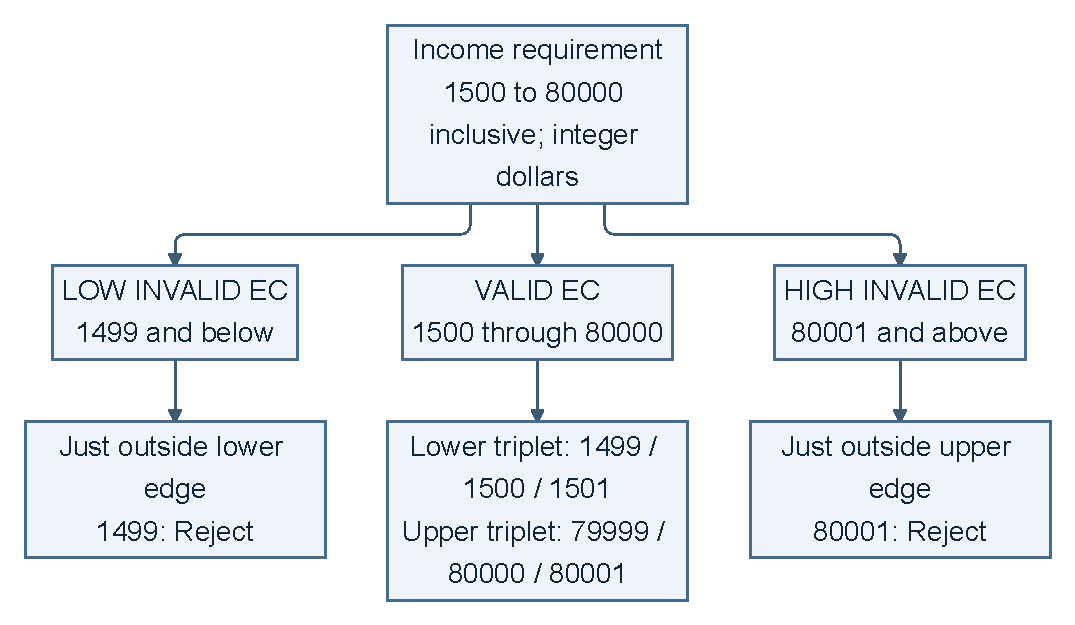
\includegraphics[width=316.48pt]{images/fig-037.pdf}
\captionof{figure}{see the mortgage-income partitions and their edges}\end{minipage}\par\smallskip

\begin{studycolumns}
\vspace{0pt}



\begin{quote}\small\color{navy}
For \textbf{each boundary of each range-of-values EC}, choose \textbf{three} values: one \textbf{on-the-boundary}, one \textbf{just-below}, one \textbf{just-above}. The size of the "just" step depends on the \textbf{unit} of the value.

\end{quote}
\textbf{In the lecture's terminology}, range-of-values parameters include integer counts. ``Discrete values'' means \textbf{unordered categories} such as Person/\allowbreak{}Company and HDB/\allowbreak{}Condo, which have no numeric BVs. Integer quantities such as mortgage count \textbf{do} have BVs.

\textbf{Worked BVs (full triplets, with the lecture's reduced valid/\allowbreak{}invalid selection):}
\end{studycolumns}


{\fontsize{9}{11}\selectfont
\begin{longtable}{L{\dimexpr 0.21399\linewidth-8.56pt\relax}L{\dimexpr 0.20246\linewidth-8.10pt\relax}L{\dimexpr 0.20697\linewidth-8.28pt\relax}L{\dimexpr 0.18829\linewidth-7.53pt\relax}L{\dimexpr 0.18829\linewidth-7.53pt\relax}}
\toprule
\rowcolor{ice}\textbf{Requirement} & \textbf{Lower boundary} & \textbf{Upper boundary} & \textbf{Valid BVs} & \textbf{Invalid BVs} \\
\midrule\endfirsthead
\toprule\rowcolor{ice}\textbf{Requirement} & \textbf{Lower boundary} & \textbf{Upper boundary} & \textbf{Valid BVs} & \textbf{Invalid BVs} \\
\midrule\endhead
\multicolumn{5}{r}{\scriptsize Continued on next page}\\\endfoot
\bottomrule\endlastfoot
Income 1500--80000 & 1499, \textbf{1500}, 1501 & 79999, \textbf{80000}, 80001 & \{1500, 80000\} & \{1499, 80001\} \\
\#mortgages 0--5 & \textbf{\ensuremath{-}1}, 0, 1 & 4, \textbf{5}, 6 & \{0, 5\} & \{\ensuremath{-}1, 6\} \\
Password length 4--8 & 3, \textbf{4}, 5 & 7, \textbf{8}, 9 & \{4, 8\} & \{3, 9\} \\
Hiring age 0--15 & \ensuremath{-}1, \textbf{0}, 1 & 14, \textbf{15}, 16 & \{0, 15\} (see de-dup below) & \{\ensuremath{-}1, 100\} \\
Hiring age 16--17 & 15, \textbf{16}, 17 & 16, \textbf{17}, 18 & \ldots{} & \ldots{} \\
Hiring age 18--54 & 17, \textbf{18}, 19 & 53, \textbf{54}, 55 & \ldots{} & \ldots{} \\
Hiring age 55--99 & 54, \textbf{55}, 56 & 98, \textbf{99}, 100 & \ldots{} & \ldots{} \\
\end{longtable}
}

\begin{studycolumns}
\vspace{0pt}

Following the \textbf{course's reduced BV selection}, the hiring sets are: \textbf{valid BVs = \{0, 15, 16, 17, 18, 54, 55, 99\}}; \textbf{invalid BVs = \{\ensuremath{-}1, 100\}}.

\textbf{The course's test-reduction rule (L18, pp. 11--15):}


\begin{quote}\small\color{navy}
Remove the just-below /\allowbreak{} just-above value from an EC's BVs (do \textbf{not} create a duplicate test case) if that value \textbf{falls into another EC} --- including the \emph{current} EC.

\end{quote}
Concretely: a just-below/\allowbreak{}just-above value is used as an \textbf{invalid test value only if it lies outside all valid ECs}. If it lands in another valid EC, that EC's own on-the-boundary value already covers it. (For 0--15, 1 is omitted because it stays inside the same EC; 16 is already a boundary of the next EC.) This is \textbf{more than removing equal duplicate values}: the slides also omit distinct interior neighbours. State the full triplets when asked for BVs, then identify the reduced test selection. Keeping all distinct triplet values is a valid stronger test suite; do not claim those values are duplicates.

\needspace{4\baselineskip}
\subsection*{13.6 Designing test cases from BVs}
\sectionlabel{h-136-designing-test-cases-from-bvs}
Same two rules as ECs, with BVs supplying the values:

\begin{itemize}
\item \textbf{Valid test cases:} combination of \textbf{on-the-boundary (valid) values}, one from each EC, combined across parameters.
\item \textbf{Invalid test cases:} \textbf{one} just-below/\allowbreak{}just-above (invalid) value per test case, with valid values for all other parameters.
\end{itemize}
For two range parameters \emph{A} and \emph{B}, the lecture uses these three test shapes:

\begin{enumerate}
\item \textbf{Valid A + Valid B} \ensuremath{\rightarrow} combination of valid inputs.
\item \textbf{Valid A + Invalid B} \ensuremath{\rightarrow} one invalid.
\item \textbf{Invalid A + Valid B} \ensuremath{\rightarrow} one invalid.
\end{enumerate}
\needspace{4\baselineskip}
\subsection*{13.7 Worked full example --- Mortgage application}
\sectionlabel{h-137-worked-full-example--mortgage-application}
\textbf{Requirements}

\begin{itemize}
\item Income must be \textbf{\$1500--\$80000/\allowbreak{}month} (L17/\allowbreak{}L18 worked problem, not L16's separate \$8000 example).
\item Number of mortgages per applicant must be \textbf{0--5}.
\item Only \textbf{Person} applicants are approved.
\item Only \textbf{HDB} and \textbf{Condo} properties are approved.
\end{itemize}
\textbf{ECs}
\end{studycolumns}


{\fontsize{9}{11}\selectfont
\begin{longtable}{L{\dimexpr 0.21333\linewidth-6.83pt\relax}L{\dimexpr 0.21333\linewidth-6.83pt\relax}L{\dimexpr 0.24633\linewidth-7.88pt\relax}L{\dimexpr 0.32702\linewidth-10.46pt\relax}}
\toprule
\rowcolor{ice}\textbf{Parameter} & \textbf{Valid EC(s)} & \textbf{Invalid EC(s)} & \textbf{BVs} \\
\midrule\endfirsthead
\toprule\rowcolor{ice}\textbf{Parameter} & \textbf{Valid EC(s)} & \textbf{Invalid EC(s)} & \textbf{BVs} \\
\midrule\endhead
\multicolumn{4}{r}{\scriptsize Continued on next page}\\\endfoot
\bottomrule\endlastfoot
Income & 1500--80000 & \ensuremath{\leq}1499 ; \ensuremath{\geq}80001 & valid \{1500, 80000\}; invalid \{1499, 80001\} \\
\#mortgage & 0--5 & \ensuremath{\leq}\ensuremath{-}1 ; \ensuremath{\geq}6 & valid \{0, 5\}; invalid \{\ensuremath{-}1, 6\} (you may additionally enumerate 1--4) \\
Applicant type & \{Person\} & \{Company, Trust, \ldots{}\} & none (discrete) \\
Property type & \{HDB, Condo\} & \{Townhouse, MobileHome, \ldots{}\} & none (discrete) \\
\end{longtable}
}

\textbf{Valid test cases} (combining valid values; enumerating the small discrete/\allowbreak{}range ECs)




{\fontsize{9}{11}\selectfont
\begin{longtable}{L{\dimexpr 0.07749\linewidth-3.72pt\relax}L{\dimexpr 0.18450\linewidth-8.86pt\relax}L{\dimexpr 0.18450\linewidth-8.86pt\relax}L{\dimexpr 0.18450\linewidth-8.86pt\relax}L{\dimexpr 0.18450\linewidth-8.86pt\relax}L{\dimexpr 0.18450\linewidth-8.86pt\relax}}
\toprule
\rowcolor{ice}\textbf{\#} & \textbf{Income} & \textbf{\#mortgage} & \textbf{Applicant} & \textbf{Property} & \textbf{Expected} \\
\midrule\endfirsthead
\toprule\rowcolor{ice}\textbf{\#} & \textbf{Income} & \textbf{\#mortgage} & \textbf{Applicant} & \textbf{Property} & \textbf{Expected} \\
\midrule\endhead
\multicolumn{6}{r}{\scriptsize Continued on next page}\\\endfoot
\bottomrule\endlastfoot
1 & \$1500 & 0 & Person & Condo & Approval \\
2 & \$2000 & 1 & Person & Condo & Approval \\
3 & \$5000 & 2 & Person & Condo & Approval \\
4 & \$12345 & 3 & Person & HDB & Approval \\
5 & \$76543 & 4 & Person & HDB & Approval \\
6 & \$80000 & 5 & Person & HDB & Approval \\
\end{longtable}
}


\begin{quote}\small\color{navy}
Note how one row already covers the single valid EC of \textbf{every} parameter (the lecture's point), and the remaining rows exist only to enumerate the small ECs' values.

\end{quote}
\textbf{Invalid test cases} (exactly one invalid per row, everything else valid)




{\fontsize{9}{11}\selectfont
\begin{longtable}{L{\dimexpr 0.07749\linewidth-3.72pt\relax}L{\dimexpr 0.18450\linewidth-8.86pt\relax}L{\dimexpr 0.18450\linewidth-8.86pt\relax}L{\dimexpr 0.18450\linewidth-8.86pt\relax}L{\dimexpr 0.18450\linewidth-8.86pt\relax}L{\dimexpr 0.18450\linewidth-8.86pt\relax}}
\toprule
\rowcolor{ice}\textbf{\#} & \textbf{Income} & \textbf{\#mortgage} & \textbf{Applicant} & \textbf{Property} & \textbf{Expected} \\
\midrule\endfirsthead
\toprule\rowcolor{ice}\textbf{\#} & \textbf{Income} & \textbf{\#mortgage} & \textbf{Applicant} & \textbf{Property} & \textbf{Expected} \\
\midrule\endhead
\multicolumn{6}{r}{\scriptsize Continued on next page}\\\endfoot
\bottomrule\endlastfoot
7 & \textbf{\$100} & 1 & Person & Condo & Reject \\
8 & \textbf{\$81000} & 2 & Person & HDB & Reject \\
9 & \$5000 & \textbf{\ensuremath{-}1} & Person & Condo & Reject \\
10 & \$10000 & \textbf{8} & Person & HDB & Reject \\
11 & \$12345 & 3 & \textbf{Company} & HDB & Reject \\
12 & \$76543 & 4 & Person & \textbf{Mobilehome} & Reject \\
\end{longtable}
}

\textbf{Avoid:} a row containing low income, eight mortgages, Company and Mobilehome simultaneously. Rejection cannot isolate which invalid class was exercised.


\Needspace{4\baselineskip}
\subsection*{13.8 Summary table (put this in your head --- it is a slide)}
\sectionlabel{h-138-summary-table-put-this-in-your-head--it-is-a-slide}


{\fontsize{9}{11}\selectfont
\begin{longtable}{L{\dimexpr 0.22429\linewidth-5.38pt\relax}L{\dimexpr 0.47432\linewidth-11.38pt\relax}L{\dimexpr 0.30138\linewidth-7.23pt\relax}}
\toprule
\rowcolor{ice}\textbf{} & \textbf{Range of values} & \textbf{Discrete values} \\
\midrule\endfirsthead
\toprule\rowcolor{ice}\textbf{} & \textbf{Range of values} & \textbf{Discrete values} \\
\midrule\endhead
\multicolumn{3}{r}{\scriptsize Continued on next page}\\\endfoot
\bottomrule\endlastfoot
\textbf{ECs} & ONE or more valid EC; \textbf{TWO} invalid ECs & ONE valid EC; ONE invalid EC \\
\textbf{BVs} & For each EC: lower boundary \ensuremath{\rightarrow} on /\allowbreak{} just-below /\allowbreak{} just-above; upper boundary \ensuremath{\rightarrow} on /\allowbreak{} just-below /\allowbreak{} just-above & \textbf{NO boundary values} \\
\end{longtable}
}

\begin{studycolumns}
\vspace{0pt}


\begin{quote}\small\color{navy}
\textbf{Trap \#1 (off-by-one).} For \code{0 \ensuremath{\leq} x \ensuremath{\leq} 5}, BVs are \textbf{\ensuremath{-}1, 0, 1} and \textbf{4, 5, 6} --- \emph{not} 0, 0.5, 1 (that is only for continuous/\allowbreak{}real-valued inputs where the unit allows halves).


\textbf{Endpoint check:} inclusive endpoints are valid; classify each neighbour against the specification, not merely its position in a triplet.

\textbf{Adjacent ECs:} deduplicate shared boundary/neighbour values; do not repeat the same input for both classes.


\textbf{Sensor check:} distinguish out-of-range input from in-range-but-business-rejected readings (Section 13.9).

\end{quote}
\needspace{4\baselineskip}
\subsection*{13.9 Worked example --- GES silo (Tutorial 8)}
\sectionlabel{h-139-worked-example--ges-silo-tutorial-8}
\textbf{Given:} humidity 0--100\%, normal 35--50\%; temperature \ensuremath{-}10--100 \textdegree{}C, normal 40--60 \textdegree{}C. The question says a silo cannot accept grain if either reading ``exceeds normal levels''.

\textbf{State the interpretation:} the solution below permits acceptance only when \textbf{both readings are inside their inclusive normal ranges}. The wording does not explicitly resolve below-normal readings. Confirm that interpretation with the client; if ``exceeds'' means only above the upper bound, the below-normal oracle changes. Assume integer percentage points and whole degrees for \ensuremath{\pm}1 BVs. Real-valued sensors require a specified resolution; \ensuremath{-}10 \textdegree{}C here is a stated input limit, not a universal physical minimum.
\end{studycolumns}


{\fontsize{9}{11}\selectfont
\begin{longtable}{L{\dimexpr 0.21809\linewidth-6.98pt\relax}L{\dimexpr 0.24919\linewidth-7.97pt\relax}L{\dimexpr 0.28620\linewidth-9.16pt\relax}L{\dimexpr 0.24652\linewidth-7.89pt\relax}}
\toprule
\rowcolor{ice}\textbf{Parameter} & \textbf{Valid normal input: permit acceptance} & \textbf{Valid sensor input: block acceptance} & \textbf{Outside stated sensor range} \\
\midrule\endfirsthead
\toprule\rowcolor{ice}\textbf{Parameter} & \textbf{Valid normal input: permit acceptance} & \textbf{Valid sensor input: block acceptance} & \textbf{Outside stated sensor range} \\
\midrule\endhead
\multicolumn{4}{r}{\scriptsize Continued on next page}\\\endfoot
\bottomrule\endlastfoot
Humidity & 35--50 & 0--34; 51--100 & \ensuremath{\leq}\ensuremath{-}1; \ensuremath{\geq}101 \\
Temperature & 40--60 & \ensuremath{-}10--39; 61--100 & \ensuremath{\leq}\ensuremath{-}11; \ensuremath{\geq}101 \\
\end{longtable}
}

``Valid sensor input'' and ``eligible to accept grain'' are different predicates. The three in-range ECs have specified business outcomes under the stated interpretation. Out-of-range input needs a validation policy; the tutorial does \textbf{not} specify an error code, message or recovery action.

\textbf{Full boundary triplets for all in-range ECs:}




{\fontsize{9}{11}\selectfont
\begin{longtable}{L{\dimexpr 0.21789\linewidth-5.23pt\relax}L{\dimexpr 0.32277\linewidth-7.75pt\relax}L{\dimexpr 0.45934\linewidth-11.02pt\relax}}
\toprule
\rowcolor{ice}\textbf{Parameter} & \textbf{Lower/\allowbreak{}upper boundaries of its ECs} & \textbf{Triplets (on \ensuremath{\pm}1)} \\
\midrule\endfirsthead
\toprule\rowcolor{ice}\textbf{Parameter} & \textbf{Lower/\allowbreak{}upper boundaries of its ECs} & \textbf{Triplets (on \ensuremath{\pm}1)} \\
\midrule\endhead
\multicolumn{3}{r}{\scriptsize Continued on next page}\\\endfoot
\bottomrule\endlastfoot
Humidity & 0, 34, 35, 50, 51, 100 & (\ensuremath{-}1,0,1); (33,34,35); (34,35,36); (49,50,51); (50,51,52); (99,100,101) \\
Temperature & \ensuremath{-}10, 39, 40, 60, 61, 100 & (\ensuremath{-}11,\ensuremath{-}10,\ensuremath{-}9); (38,39,40); (39,40,41); (59,60,61); (60,61,62); (99,100,101) \\
\end{longtable}
}

Following the lecture's reduced BV selection gives humidity \code{\{\ensuremath{-}1,\allowbreak{}0,\allowbreak{}34,\allowbreak{}35,\allowbreak{}50,\allowbreak{}51,\allowbreak{}100,\allowbreak{}101\}} and temperature \code{\{\ensuremath{-}11,\allowbreak{}\ensuremath{-}10,\allowbreak{}39,\allowbreak{}40,\allowbreak{}60,\allowbreak{}61,\allowbreak{}100,\allowbreak{}101\}}. Interior neighbours may additionally be retained for stronger boundary checks.




{\fontsize{9}{11}\selectfont
\begin{longtable}{L{\dimexpr 0.09692\linewidth-3.10pt\relax}L{\dimexpr 0.23077\linewidth-7.38pt\relax}L{\dimexpr 0.23077\linewidth-7.38pt\relax}L{\dimexpr 0.44155\linewidth-14.13pt\relax}}
\toprule
\rowcolor{ice}\textbf{\#} & \textbf{Humidity} & \textbf{Temperature} & \textbf{Expected outcome under the stated interpretation} \\
\midrule\endfirsthead
\toprule\rowcolor{ice}\textbf{\#} & \textbf{Humidity} & \textbf{Temperature} & \textbf{Expected outcome under the stated interpretation} \\
\midrule\endhead
\multicolumn{4}{r}{\scriptsize Continued on next page}\\\endfoot
\bottomrule\endlastfoot
1 & 35 & 40 & Permit acceptance: both lower normal boundaries \\
2 & 50 & 60 & Permit acceptance: both upper normal boundaries \\
3 & 0 & 45 & Block: humidity below normal, valid sensor input \\
4 & 34 & 45 & Block: humidity just below normal \\
5 & 51 & 45 & Block: humidity just above normal \\
6 & 100 & 45 & Block: humidity above normal, at sensor limit \\
7 & 45 & \ensuremath{-}10 & Block: temperature below normal, at sensor limit \\
8 & 45 & 39 & Block: temperature just below normal \\
9 & 45 & 61 & Block: temperature just above normal \\
10 & 45 & 100 & Block: temperature above normal, at sensor limit \\
11 & \ensuremath{-}1 & 45 & Out-of-range humidity; validation response TBD \\
12 & 101 & 45 & Out-of-range humidity; validation response TBD \\
13 & 45 & \ensuremath{-}11 & Out-of-range temperature; validation response TBD \\
14 & 45 & 101 & Out-of-range temperature; validation response TBD \\
\end{longtable}
}

Rows 3--10 isolate one abnormal reading; rows 11--14 isolate one invalid sensor input. Acceptance also depends on capacity/\allowbreak{}type/\allowbreak{}grade in the complete GES, but Tutorial 8 isolates the sensor rule.


